\documentclass[a4paper,11pt]{article}
\usepackage[pdftex]{graphicx}
\usepackage{biblatex}
\addbibresource{mybib.bib}

\author{T. Kooij}
\title{Time walk}

\begin{document}
\maketitle

\section{Abstract}

\section{Introduction}
Time walk is an instrumental shift in measured time using a detection threshold in scintillator-PMT systems. Time walk is caused by a difference in rise time for coincident signals of different amplitude.

\begin{figure}[h!]
  \centering
    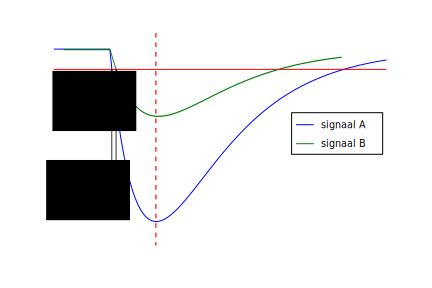
\includegraphics[width=0.8\textwidth]{fig17_1.pdf}
  \caption{Time walk between coincident signal with different pulseheight. \textit {Recreated from figure 17.1 of \cite{Leo:1987} } }
  \label{fig_timewalk}
\end{figure}

In figure \ref{fig_timewalk} the signals are caused by coincident particles in a scintillator connected to a PMT. Signal A crosses the threshold at time $t_A$ and signal B crosses the threshold at $t_B$. The pulsesheight for Signal A is larger and thus the rise-time is smaller and the signal crosses the threshold earlier. This results in a time difference $t_{walk} = t_B - t_A$.

In HiSPARC detectors we consider two regimes in the pulseintegral histogram. An exponentially decaying part that is considered to be dominated by detected gamma rays and a gaussian convoluted landau part that is considered to be dominated by detected charged leptons.

\begin{figure}[h!]
  \centering
    \includegraphics[width=0.8\textwidth]{pulseheight.png}
  \caption{Pulseintegral histogram for WEETIKVEEL}
  \label{fig_hist}
\end{figure}

The two parts can also be distinguished based on pulseheights. In the histogram shown above (figure \ref{fig_hist}), the gamma part has pulseheights below 120 ADC. Pulseheights above 200 ADC are considered to below to the charged lepton part \cite{Pennink:2010}.

\begin{figure}[h!]
  \centering
    \includegraphics[width=0.8\textwidth]{delta_t.png}
  \caption{Time difference t1 - t2. Station 501 (nikhef), Jan 1st, 2014 - May 31st, 2014. ph1 > 200 (high, charged lepton), 20 < ph2 < 120 (low, gamma). Figure created by lio\_project timewalk s501\_delta\_t.py}
  \label{fig_delta_t}
\end{figure}

The arrival time difference ($t_1 - t_2$) of particles particles in the charged lepton part (corresponding to $t_1$) and gamma's (corresponding to $t_2$) are shown in figure \ref{fig_delta_t}. The skewness of the histogram is typical. The distribution is skewed towards the times resulting from lower pulseheights ($t_2$). Here the distribution is skewed to the left.

Figure \ref{fig_delta_t} resembles arrival time distributions in \i{time of flight} (TOF) detectors before correcting for time walk. In TOF experiments the skewness disappears after time walk correction and the distribution becomes symmetric.
\subsection{Goal}
In this paper the time walk correction for the dataset shown above is calculated and it the contribution of time walk correction to the skewness of the arrival time distribution is investigated. 

\section{Time walk correction}

Time walk has been measured and succesfully parametrised with respect to pulseintegral in \cite{Brown:1983ka} and \cite{Smith:2002}
\begin{equation}
t = t_0 + \frac{ a }{\sqrt{x}}
\end{equation}
where x is the pulseintegral, $t_0$ and a are to be fitted using experimental data.

Note time shift $t_0$ is needed for analysis and fitting only. It will cancel out in time differences calculated after correction.

Good correlation with experimental data is quoted by \cite{Brown:1983ka}. However \cite{Smith:2002} specifically considers signals where the PM is not yet saturated:
\begin{equation}
t = t_0 + \frac{a}{x^b}
\end{equation}
where x is the pulseintegral, $t_0$, a and b are to be fitted using experimental data.

We will fit both models to our data.

\section{Time walk analysis in a HiSPARC station}
\subsection{Description of the dataset}
The dataset consists of events from HiSPARC station 501 (Nikhef) from January until May 2014. \footnote{The dataset is created by {\textit{lio\_project timewalk read\_ESD.py}}}

Time difference between detector 1 and 2 (distance 10 m) is considered for events where $pulseheight_1 > 200$ ADC and $pulseheight_2 < 120$ ADC (but above the threshold: $pulseheight_2 > 20$ ADC). These limits have been set by \cite{Pennink:2010}. Signal 1 is dominated by charged leptons. Signal 2 is dominated by gamma's.

A histogram of $t_1 - t_2 $ for these events is shown in figure \ref{fig_delta_t}.



\subsection{Binning}

The dataset \footnote{Binning of the data is done by {\textit{lio\_project timewalk walk.py}}}
is binned using $pulseheight_2$ (\textit{low} pulseheight). From 20 ADC to 120 ADC we use 40 bins of width 2.5 ADC. (bins = 20, 22.5, 25.0, ... 120. (ADC)).

\begin{figure}[h!]
  \centering
    \includegraphics[width=0.8\textwidth]{delta_t.png}
  \caption{DIFFERENT FIGURE GOES HERE Figure created by lio\_project timewalk walk.py}
  \label{fig_bin}
\end{figure}

For each bin a histogram is created and a histogram is fitted. Figure \ref{bin_fit} shows a typical histogram with fit. $Chi^2$ are average XXX, sigma = XXX.



\printbibliography
\end{document}
